%%%%%%%%%%%%%%%%%%%%%%%%%%%%%%%%%%%%%%%%%
% The Legrand Orange Book
% LaTeX Template
% Version 2.0 (9/2/15)
%
% This template has been downloaded from:
% http://www.LaTeXTemplates.com
%
% Mathias Legrand (legrand.mathias@gmail.com) with modifications by:
% Vel (vel@latextemplates.com)
%
% License:
% CC BY-NC-SA 3.0 (http://creativecommons.org/licenses/by-nc-sa/3.0/)
%
% Compiling this template:
% This template uses biber for its bibliography and makeindex for its index.
% When you first open the template, compile it from the command line with the 
% commands below to make sure your LaTeX distribution is configured correctly:
%
% 1) pdflatex main
% 2) makeindex main.idx -s StyleInd.ist
% 3) biber main
% 4) pdflatex main x 2
%
% After this, when you wish to update the bibliography/index use the appropriate
% command above and make sure to compile with pdflatex several times 
% afterwards to propagate your changes to the document.
%
% This template also uses a number of packages which may need to be
% updated to the newest versions for the template to compile. It is strongly
% recommended you update your LaTeX distribution if you have any
% compilation errors.
%
% Important note:
% Chapter heading images should have a 2:1 width:height ratio,
% e.g. 920px width and 460px height.
%
%%%%%%%%%%%%%%%%%%%%%%%%%%%%%%%%%%%%%%%%%

%you need to compile this template up to 3 times!

%----------------------------------------------------------------------------------------
%	PACKAGES AND OTHER DOCUMENT CONFIGURATIONS
%----------------------------------------------------------------------------------------

\documentclass[11pt,fleqn]{book} % Default font size and left-justified equations
%\usepackage[toc,page]{appendix}
%----------------------------------------------------------------------------------------

%%%%%%%%%%%%%%%%%%%%%%%%%%%%%%%%%%%%%%%%%
% The Legrand Orange Book
% Structural Definitions File
% Version 2.0 (9/2/15)
%
% Original author:
% Mathias Legrand (legrand.mathias@gmail.com) with modifications by:
% Vel (vel@latextemplates.com)
% 
% This file has been downloaded from:
% http://www.LaTeXTemplates.com
%
% License:
% CC BY-NC-SA 3.0 (http://creativecommons.org/licenses/by-nc-sa/3.0/)
%
%%%%%%%%%%%%%%%%%%%%%%%%%%%%%%%%%%%%%%%%%

%----------------------------------------------------------------------------------------
%	VARIOUS REQUIRED PACKAGES AND CONFIGURATIONS
%----------------------------------------------------------------------------------------

\usepackage[top=3cm,bottom=3cm,left=3cm,right=3cm,headsep=10pt,a4paper]{geometry} % Page margins

\usepackage{graphicx} % Required for including pictures
\graphicspath{{Pictures/}} % Specifies the directory where pictures are stored

\usepackage{lipsum} % Inserts dummy text

\usepackage{tikz} % Required for drawing custom shapes

\usepackage[english]{babel} % English language/hyphenation

\usepackage{enumitem} % Customize lists
\setlist{nolistsep} % Reduce spacing between bullet points and numbered lists

\usepackage{booktabs} % Required for nicer horizontal rules in tables

\usepackage{xcolor} % Required for specifying colors by name
\definecolor{ocre}{RGB}{243,102,25} % Define the orange color used for highlighting throughout the book

%----------------------------------------------------------------------------------------
%	FONTS
%----------------------------------------------------------------------------------------

\usepackage{avant} % Use the Avantgarde font for headings
%\usepackage{times} % Use the Times font for headings
\usepackage{mathptmx} % Use the Adobe Times Roman as the default text font together with math symbols from the Sym­bol, Chancery and Com­puter Modern fonts

\usepackage{microtype} % Slightly tweak font spacing for aesthetics
\usepackage[utf8]{inputenc} % Required for including letters with accents
\usepackage[T1]{fontenc} % Use 8-bit encoding that has 256 glyphs

%----------------------------------------------------------------------------------------
%	BIBLIOGRAPHY AND INDEX
%----------------------------------------------------------------------------------------

\usepackage[style=alphabetic,citestyle=numeric,sorting=nyt,sortcites=true,autopunct=true,babel=hyphen,hyperref=true,abbreviate=false,backref=true,backend=biber]{biblatex}
\addbibresource{bibliography.bib} % BibTeX bibliography file
\defbibheading{bibempty}{}

\usepackage{calc} % For simpler calculation - used for spacing the index letter headings correctly
\usepackage{makeidx} % Required to make an index
\makeindex % Tells LaTeX to create the files required for indexing

%----------------------------------------------------------------------------------------
%	MAIN TABLE OF CONTENTS
%----------------------------------------------------------------------------------------

\usepackage{titletoc} % Required for manipulating the table of contents

\contentsmargin{0cm} % Removes the default margin

% Part text styling
\titlecontents{part}[0cm]
{\addvspace{20pt}\centering\large\bfseries}
{}
{}
{}

% Chapter text styling
\titlecontents{chapter}[1.25cm] % Indentation
{\addvspace{12pt}\large\sffamily\bfseries} % Spacing and font options for chapters
{\color{ocre!60}\contentslabel[\Large\thecontentslabel]{1.25cm}\color{ocre}} % Chapter number
{\color{ocre}}  
{\color{ocre!60}\normalsize\;\titlerule*[.5pc]{.}\;\thecontentspage} % Page number

% Section text styling
\titlecontents{section}[1.25cm] % Indentation
{\addvspace{3pt}\sffamily\bfseries} % Spacing and font options for sections
{\contentslabel[\thecontentslabel]{1.25cm}} % Section number
{}
{\hfill\color{black}\thecontentspage} % Page number
[]

% Subsection text styling
\titlecontents{subsection}[1.25cm] % Indentation
{\addvspace{1pt}\sffamily\small} % Spacing and font options for subsections
{\contentslabel[\thecontentslabel]{1.25cm}} % Subsection number
{}
{\ \titlerule*[.5pc]{.}\;\thecontentspage} % Page number
[]

% List of figures
\titlecontents{figure}[0em]
{\addvspace{-5pt}\sffamily}
{\thecontentslabel\hspace*{1em}}
{}
{\ \titlerule*[.5pc]{.}\;\thecontentspage}
[]

% List of tables
\titlecontents{table}[0em]
{\addvspace{-5pt}\sffamily}
{\thecontentslabel\hspace*{1em}}
{}
{\ \titlerule*[.5pc]{.}\;\thecontentspage}
[]

%----------------------------------------------------------------------------------------
%	MINI TABLE OF CONTENTS IN PART HEADS
%----------------------------------------------------------------------------------------

% Chapter text styling
\titlecontents{lchapter}[0em] % Indenting
{\addvspace{15pt}\large\sffamily\bfseries} % Spacing and font options for chapters
{\color{ocre}\contentslabel[\Large\thecontentslabel]{1.25cm}\color{ocre}} % Chapter number
{}  
{\color{ocre}\normalsize\sffamily\bfseries\;\titlerule*[.5pc]{.}\;\thecontentspage} % Page number

% Section text styling
\titlecontents{lsection}[0em] % Indenting
{\sffamily\small} % Spacing and font options for sections
{\contentslabel[\thecontentslabel]{1.25cm}} % Section number
{}
{}

% Subsection text styling
\titlecontents{lsubsection}[.5em] % Indentation
{\normalfont\footnotesize\sffamily} % Font settings
{}
{}
{}

%----------------------------------------------------------------------------------------
%	PAGE HEADERS
%----------------------------------------------------------------------------------------

\usepackage{fancyhdr} % Required for header and footer configuration

\pagestyle{fancy}
\renewcommand{\chaptermark}[1]{\markboth{\sffamily\normalsize\bfseries\chaptername\ \thechapter.\ #1}{}} % Chapter text font settings
\renewcommand{\sectionmark}[1]{\markright{\sffamily\normalsize\thesection\hspace{5pt}#1}{}} % Section text font settings
\fancyhf{} \fancyhead[LE,RO]{\sffamily\normalsize\thepage} % Font setting for the page number in the header
\fancyhead[LO]{\rightmark} % Print the nearest section name on the left side of odd pages
\fancyhead[RE]{\leftmark} % Print the current chapter name on the right side of even pages
\renewcommand{\headrulewidth}{0.5pt} % Width of the rule under the header
\addtolength{\headheight}{2.5pt} % Increase the spacing around the header slightly
\renewcommand{\footrulewidth}{0pt} % Removes the rule in the footer
\fancypagestyle{plain}{\fancyhead{}\renewcommand{\headrulewidth}{0pt}} % Style for when a plain pagestyle is specified

% Removes the header from odd empty pages at the end of chapters
\makeatletter
\renewcommand{\cleardoublepage}{
\clearpage\ifodd\c@page\else
\hbox{}
\vspace*{\fill}
\thispagestyle{empty}
\newpage
\fi}

%----------------------------------------------------------------------------------------
%	THEOREM STYLES
%----------------------------------------------------------------------------------------

\usepackage{amsmath,amsfonts,amssymb,amsthm} % For math equations, theorems, symbols, etc

\newcommand{\intoo}[2]{\mathopen{]}#1\,;#2\mathclose{[}}
\newcommand{\ud}{\mathop{\mathrm{{}d}}\mathopen{}}
\newcommand{\intff}[2]{\mathopen{[}#1\,;#2\mathclose{]}}
\newtheorem{notation}{Notation}[chapter]

% Boxed/framed environments
\newtheoremstyle{ocrenumbox}% % Theorem style name
{0pt}% Space above
{0pt}% Space below
{\normalfont}% % Body font
{}% Indent amount
{\small\bf\sffamily\color{ocre}}% % Theorem head font
{\;}% Punctuation after theorem head
{0.25em}% Space after theorem head
{\small\sffamily\color{ocre}\thmname{#1}\nobreakspace\thmnumber{\@ifnotempty{#1}{}\@upn{#2}}% Theorem text (e.g. Theorem 2.1)
\thmnote{\nobreakspace\the\thm@notefont\sffamily\bfseries\color{black}---\nobreakspace#3.}} % Optional theorem note
\renewcommand{\qedsymbol}{$\blacksquare$}% Optional qed square

\newtheoremstyle{blacknumex}% Theorem style name
{5pt}% Space above
{5pt}% Space below
{\normalfont}% Body font
{} % Indent amount
{\small\bf\sffamily}% Theorem head font
{\;}% Punctuation after theorem head
{0.25em}% Space after theorem head
{\small\sffamily{\tiny\ensuremath{\blacksquare}}\nobreakspace\thmname{#1}\nobreakspace\thmnumber{\@ifnotempty{#1}{}\@upn{#2}}% Theorem text (e.g. Theorem 2.1)
\thmnote{\nobreakspace\the\thm@notefont\sffamily\bfseries---\nobreakspace#3.}}% Optional theorem note

\newtheoremstyle{blacknumbox} % Theorem style name
{0pt}% Space above
{0pt}% Space below
{\normalfont}% Body font
{}% Indent amount
{\small\bf\sffamily}% Theorem head font
{\;}% Punctuation after theorem head
{0.25em}% Space after theorem head
{\small\sffamily\thmname{#1}\nobreakspace\thmnumber{\@ifnotempty{#1}{}\@upn{#2}}% Theorem text (e.g. Theorem 2.1)
\thmnote{\nobreakspace\the\thm@notefont\sffamily\bfseries---\nobreakspace#3.}}% Optional theorem note

% Non-boxed/non-framed environments
\newtheoremstyle{ocrenum}% % Theorem style name
{5pt}% Space above
{5pt}% Space below
{\normalfont}% % Body font
{}% Indent amount
{\small\bf\sffamily\color{ocre}}% % Theorem head font
{\;}% Punctuation after theorem head
{0.25em}% Space after theorem head
{\small\sffamily\color{ocre}\thmname{#1}\nobreakspace\thmnumber{\@ifnotempty{#1}{}\@upn{#2}}% Theorem text (e.g. Theorem 2.1)
\thmnote{\nobreakspace\the\thm@notefont\sffamily\bfseries\color{black}---\nobreakspace#3.}} % Optional theorem note
\renewcommand{\qedsymbol}{$\blacksquare$}% Optional qed square
\makeatother

% Defines the theorem text style for each type of theorem to one of the three styles above
\newcounter{dummy} 
\numberwithin{dummy}{section}
\theoremstyle{ocrenumbox}
\newtheorem{theoremeT}[dummy]{Theorem}
\newtheorem{problem}{Problem}[chapter]
\newtheorem{exerciseT}{Exercise}[chapter]
\theoremstyle{blacknumex}
\newtheorem{exampleT}{Example}[chapter]
\theoremstyle{blacknumbox}
\newtheorem{vocabulary}{Vocabulary}[chapter]
\newtheorem{definitionT}{Definition}[section]
\newtheorem{corollaryT}[dummy]{Corollary}
\theoremstyle{ocrenum}
\newtheorem{proposition}[dummy]{Proposition}

%----------------------------------------------------------------------------------------
%	DEFINITION OF COLORED BOXES
%----------------------------------------------------------------------------------------

\RequirePackage[framemethod=default]{mdframed} % Required for creating the theorem, definition, exercise and corollary boxes

% Theorem box
\newmdenv[skipabove=7pt,
skipbelow=7pt,
backgroundcolor=black!5,
linecolor=ocre,
innerleftmargin=5pt,
innerrightmargin=5pt,
innertopmargin=5pt,
leftmargin=0cm,
rightmargin=0cm,
innerbottommargin=5pt]{tBox}

% Exercise box	  
\newmdenv[skipabove=7pt,
skipbelow=7pt,
rightline=false,
leftline=true,
topline=false,
bottomline=false,
backgroundcolor=ocre!10,
linecolor=ocre,
innerleftmargin=5pt,
innerrightmargin=5pt,
innertopmargin=5pt,
innerbottommargin=5pt,
leftmargin=0cm,
rightmargin=0cm,
linewidth=4pt]{eBox}	

% Definition box
\newmdenv[skipabove=7pt,
skipbelow=7pt,
rightline=false,
leftline=true,
topline=false,
bottomline=false,
linecolor=ocre,
innerleftmargin=5pt,
innerrightmargin=5pt,
innertopmargin=0pt,
leftmargin=0cm,
rightmargin=0cm,
linewidth=4pt,
innerbottommargin=0pt]{dBox}	

% Corollary box
\newmdenv[skipabove=7pt,
skipbelow=7pt,
rightline=false,
leftline=true,
topline=false,
bottomline=false,
linecolor=gray,
backgroundcolor=black!5,
innerleftmargin=5pt,
innerrightmargin=5pt,
innertopmargin=5pt,
leftmargin=0cm,
rightmargin=0cm,
linewidth=4pt,
innerbottommargin=5pt]{cBox}

% Creates an environment for each type of theorem and assigns it a theorem text style from the "Theorem Styles" section above and a colored box from above
\newenvironment{theorem}{\begin{tBox}\begin{theoremeT}}{\end{theoremeT}\end{tBox}}
\newenvironment{exercise}{\begin{eBox}\begin{exerciseT}}{\hfill{\color{ocre}\tiny\ensuremath{\blacksquare}}\end{exerciseT}\end{eBox}}				  
\newenvironment{definition}{\begin{dBox}\begin{definitionT}}{\end{definitionT}\end{dBox}}	
\newenvironment{example}{\begin{exampleT}}{\hfill{\tiny\ensuremath{\blacksquare}}\end{exampleT}}		
\newenvironment{corollary}{\begin{cBox}\begin{corollaryT}}{\end{corollaryT}\end{cBox}}	

%----------------------------------------------------------------------------------------
%	REMARK ENVIRONMENT
%----------------------------------------------------------------------------------------

\newenvironment{remark}{\par\vspace{10pt}\small % Vertical white space above the remark and smaller font size
\begin{list}{}{
\leftmargin=35pt % Indentation on the left
\rightmargin=25pt}\item\ignorespaces % Indentation on the right
\makebox[-2.5pt]{\begin{tikzpicture}[overlay]
\node[draw=ocre!60,line width=1pt,circle,fill=ocre!25,font=\sffamily\bfseries,inner sep=2pt,outer sep=0pt] at (-15pt,0pt){\textcolor{ocre}{R}};\end{tikzpicture}} % Orange R in a circle
\advance\baselineskip -1pt}{\end{list}\vskip5pt} % Tighter line spacing and white space after remark

%----------------------------------------------------------------------------------------
%	SECTION NUMBERING IN THE MARGIN
%----------------------------------------------------------------------------------------

\makeatletter
\renewcommand{\@seccntformat}[1]{\llap{\textcolor{ocre}{\csname the#1\endcsname}\hspace{1em}}}                    
\renewcommand{\section}{\@startsection{section}{1}{\z@}
{-4ex \@plus -1ex \@minus -.4ex}
{1ex \@plus.2ex }
{\normalfont\large\sffamily\bfseries}}
\renewcommand{\subsection}{\@startsection {subsection}{2}{\z@}
{-3ex \@plus -0.1ex \@minus -.4ex}
{0.5ex \@plus.2ex }
{\normalfont\sffamily\bfseries}}
\renewcommand{\subsubsection}{\@startsection {subsubsection}{3}{\z@}
{-2ex \@plus -0.1ex \@minus -.2ex}
{.2ex \@plus.2ex }
{\normalfont\small\sffamily\bfseries}}                        
\renewcommand\paragraph{\@startsection{paragraph}{4}{\z@}
{-2ex \@plus-.2ex \@minus .2ex}
{.1ex}
{\normalfont\small\sffamily\bfseries}}

%----------------------------------------------------------------------------------------
%	PART HEADINGS
%----------------------------------------------------------------------------------------

% numbered part in the table of contents
\newcommand{\@mypartnumtocformat}[2]{%
\setlength\fboxsep{0pt}%
\noindent\colorbox{ocre!20}{\strut\parbox[c][.7cm]{\ecart}{\color{ocre!70}\Large\sffamily\bfseries\centering#1}}\hskip\esp\colorbox{ocre!40}{\strut\parbox[c][.7cm]{\linewidth-\ecart-\esp}{\Large\sffamily\centering#2}}}%
%%%%%%%%%%%%%%%%%%%%%%%%%%%%%%%%%%
% unnumbered part in the table of contents
\newcommand{\@myparttocformat}[1]{%
\setlength\fboxsep{0pt}%
\noindent\colorbox{ocre!40}{\strut\parbox[c][.7cm]{\linewidth}{\Large\sffamily\centering#1}}}%
%%%%%%%%%%%%%%%%%%%%%%%%%%%%%%%%%%
\newlength\esp
\setlength\esp{4pt}
\newlength\ecart
\setlength\ecart{1.2cm-\esp}
\newcommand{\thepartimage}{}%
\newcommand{\partimage}[1]{\renewcommand{\thepartimage}{#1}}%
\def\@part[#1]#2{%
\ifnum \c@secnumdepth >-2\relax%
\refstepcounter{part}%
\addcontentsline{toc}{part}{\texorpdfstring{\protect\@mypartnumtocformat{\thepart}{#1}}{\partname~\thepart\ ---\ #1}}
\else%
\addcontentsline{toc}{part}{\texorpdfstring{\protect\@myparttocformat{#1}}{#1}}%
\fi%
\startcontents%
\markboth{}{}%
{\thispagestyle{empty}%
\begin{tikzpicture}[remember picture,overlay]%
\node at (current page.north west){\begin{tikzpicture}[remember picture,overlay]%	
\fill[ocre!20](0cm,0cm) rectangle (\paperwidth,-\paperheight);
\node[anchor=north] at (4cm,-3.25cm){\color{ocre!40}\fontsize{220}{100}\sffamily\bfseries\@Roman\c@part}; 
\node[anchor=south east] at (\paperwidth-1cm,-\paperheight+1cm){\parbox[t][][t]{8.5cm}{
\printcontents{l}{0}{\setcounter{tocdepth}{1}}%
}};
\node[anchor=north east] at (\paperwidth-1.5cm,-3.25cm){\parbox[t][][t]{15cm}{\strut\raggedleft\color{white}\fontsize{30}{30}\sffamily\bfseries#2}};
\end{tikzpicture}};
\end{tikzpicture}}%
\@endpart}
\def\@spart#1{%
\startcontents%
\phantomsection
{\thispagestyle{empty}%
\begin{tikzpicture}[remember picture,overlay]%
\node at (current page.north west){\begin{tikzpicture}[remember picture,overlay]%	
\fill[ocre!20](0cm,0cm) rectangle (\paperwidth,-\paperheight);
\node[anchor=north east] at (\paperwidth-1.5cm,-3.25cm){\parbox[t][][t]{15cm}{\strut\raggedleft\color{white}\fontsize{30}{30}\sffamily\bfseries#1}};
\end{tikzpicture}};
\end{tikzpicture}}
\addcontentsline{toc}{part}{\texorpdfstring{%
\setlength\fboxsep{0pt}%
\noindent\protect\colorbox{ocre!40}{\strut\protect\parbox[c][.7cm]{\linewidth}{\Large\sffamily\protect\centering #1\quad\mbox{}}}}{#1}}%
\@endpart}
\def\@endpart{\vfil\newpage
\if@twoside
\if@openright
\null
\thispagestyle{empty}%
\newpage
\fi
\fi
\if@tempswa
\twocolumn
\fi}

%----------------------------------------------------------------------------------------
%	CHAPTER HEADINGS
%----------------------------------------------------------------------------------------

\newcommand{\thechapterimage}{}%
\newcommand{\chapterimage}[1]{\renewcommand{\thechapterimage}{#1}}%
\def\@makechapterhead#1{%
{\parindent \z@ \raggedright \normalfont
\ifnum \c@secnumdepth >\m@ne
\if@mainmatter
\begin{tikzpicture}[remember picture,overlay]
\node at (current page.north west)
{\begin{tikzpicture}[remember picture,overlay]
\node[anchor=north west,inner sep=0pt] at (0,0) {\includegraphics[width=\paperwidth]{\thechapterimage}};
\draw[anchor=west] (\Gm@lmargin,-9cm) node [line width=2pt,rounded corners=15pt,draw=ocre,fill=white,fill opacity=0.5,inner sep=15pt]{\strut\makebox[22cm]{}};
\draw[anchor=west] (\Gm@lmargin+.3cm,-9cm) node {\huge\sffamily\bfseries\color{black}\thechapter. #1\strut};
\end{tikzpicture}};
\end{tikzpicture}
\else
\begin{tikzpicture}[remember picture,overlay]
\node at (current page.north west)
{\begin{tikzpicture}[remember picture,overlay]
\node[anchor=north west,inner sep=0pt] at (0,0) {\includegraphics[width=\paperwidth]{\thechapterimage}};
\draw[anchor=west] (\Gm@lmargin,-9cm) node [line width=2pt,rounded corners=15pt,draw=ocre,fill=white,fill opacity=0.5,inner sep=15pt]{\strut\makebox[22cm]{}};
\draw[anchor=west] (\Gm@lmargin+.3cm,-9cm) node {\huge\sffamily\bfseries\color{black}#1\strut};
\end{tikzpicture}};
\end{tikzpicture}
\fi\fi\par\vspace*{270\p@}}}

%-------------------------------------------

\def\@makeschapterhead#1{%
\begin{tikzpicture}[remember picture,overlay]
\node at (current page.north west)
{\begin{tikzpicture}[remember picture,overlay]
\node[anchor=north west,inner sep=0pt] at (0,0) {\includegraphics[width=\paperwidth]{\thechapterimage}};
\draw[anchor=west] (\Gm@lmargin,-9cm) node [line width=2pt,rounded corners=15pt,draw=ocre,fill=white,fill opacity=0.5,inner sep=15pt]{\strut\makebox[22cm]{}};
\draw[anchor=west] (\Gm@lmargin+.3cm,-9cm) node {\huge\sffamily\bfseries\color{black}#1\strut};
\end{tikzpicture}};
\end{tikzpicture}
\par\vspace*{270\p@}}
\makeatother

%----------------------------------------------------------------------------------------
%	HYPERLINKS IN THE DOCUMENTS
%----------------------------------------------------------------------------------------

\usepackage{hyperref}
\hypersetup{hidelinks,backref=true,pagebackref=true,hyperindex=true,colorlinks=false,breaklinks=true,urlcolor= ocre,bookmarks=true,bookmarksopen=false,pdftitle={Title},pdfauthor={Author}}
\usepackage{bookmark}
\bookmarksetup{
open,
numbered,
addtohook={%
\ifnum\bookmarkget{level}=0 % chapter
\bookmarksetup{bold}%
\fi
\ifnum\bookmarkget{level}=-1 % part
\bookmarksetup{color=ocre,bold}%
\fi
}
} % Insert the commands.tex file which contains the majority of the structure behind the template


%---- LKB stuff

%%My std preamble for the docs
%\selectlanguage{british}%
\usepackage[british]{babel}
\usepackage{microtype} %better text
\IfFileExists{lmodern.sty}{\usepackage{lmodern}}{} %type 1 vector font
%
\usepackage{lettrine}
\usepackage{listings} %Add list support
\usepackage{colortbl} %colors in TABLES
%\usepackage{tikz,amsmath, amssymb,bm,color}
\usepackage{nicefrac}
\usepackage{lastpage} %get last page

%COLORS
\usepackage{color}
\definecolor{lightgray}{gray}{0.8} %for colortbl
\definecolor{UniBlue}{RGB}{83,121,170}
\definecolor{deepBlue}{HTML}{000066}
\definecolor{blueBgd}{HTML}{99C8FF}
\definecolor{aBlue}{HTML}{1879F7}

%%%%%%%%%%%%%%%%%%%%%%%%%%%%%%%%%%%%%%%%%%%%%%%%%%%%%%%%%%%%%%%%%%
%FOOTNOTES
%nice look after http://www.dedoimedo.com


%%%%%%%%%%%%%%%%%%%%%%%%%%%%%%%%%%%%%%%%%%%%%%%%%%%%%%%%%%%%%%%%%%%
%TABLE SETTINGS
\usepackage{colortbl} %colors in table
\usepackage{rotating} %rotatins within tables
\usepackage{multirow}
\renewcommand{\arraystretch}{1.2} %add padding/spacing
%\usepackage{adjustbox}%rotating and fitting into page
%

\usepackage{booktabs} % To thicken table lines
%define thickness of table lines
\let\mytoprule\toprule
\renewcommand{\toprule}{\mytoprule[0.20em]}
\let\mytoprule\bottomrule
\renewcommand{\bottomrule}{\mytoprule[0.20em]}
\let\mytoprule\midrule
\renewcommand{\midrule}{\mytoprule[0.08em]}

\usepackage{spreadtab} % for simple calculations

%vertically and horizontally centered multicolumn cells with a fixed width. M{width}
%\newcolumntype{M}[1]{>{\centering\hspace{0pt}}m{#1}}
% each spanned cell has the same width. S{width of multicolumn cell}{number of spanned columns}
%\newcolumntype{S}[2]{>{\centering\hspace{0pt}}m{(#1+(2\tabcolsep+\arrayrulewidth)*(1-#2))/#2}}

%%%%%%%%%%%%%%%%%%%%%%%%%%%%%%%%%%%%%%%%%%%%%%%%%%%%%%%%%%%%%%%%%%%
%TikZ
\usepackage{tikz}

\colorlet{red}{red!50}
\colorlet{green}{green!50}
\colorlet{blue}{blue!50}
\definecolor{yellow}{HTML}{FFFF00}
\colorlet{yellow}{yellow!50}
\definecolor{fiolet}{HTML}{7030A0}
\colorlet{fiolet}{fiolet!50}
\colorlet{bgd_main}{black!50}
\colorlet{bgd}{bgd_main!75}
\colorlet{bgd2}{bgd_main!50}
\colorlet{bgd3}{bgd_main!25}
\colorlet{bgd4}{bgd_main!15}

\usetikzlibrary{shapes,arrows,calc,positioning}

%%%%%%%%%%%%%%%%%%%%%%%%%%%%%%%%%%%%%%%%%%%%%%%%%%%%%%%%%%%%%%%%%%%
% Footnotes in Figs
%\rule[raise-height]{width}{thickness}
\newcommand*{\FigFootnote}[1]{
\noindent \begin{flushleft}
\rule[0.2ex]{0.4\columnwidth}{0.5pt}
\par
\footnotesize
#1
\footnotesize
\end{flushleft}
}

%%%%%%%%%%%%%%%%%%%%%%%%%%%%%%%%%%%%%%%%%%%%%%%%%%%%%%%%%%%%%%%%%%%
%MATH, number display
%need to install siunitx, l3kernel,l3packages
\usepackage{siunitx} %this is for units display

\sisetup{per-mode=fraction, tight-spacing = true , fraction-function = \nicefrac, quotient-mode = fraction}% %nicefrac \tfrac
\sisetup{inter-unit-product = \ensuremath { { } \cdot { } } , exponent-product = \cdot }%
\sisetup{input-product=x , output-quotient =  \ensuremath { { } \times{}}} %for 1x2x3
%number grouping(3), std==true %\sisetup{group-digits = decimal} 
\sisetup{group-minimum-digits = 4} %start grouping from 4 digits, in 3 no groups
\sisetup{range-units = single,range-phrase = \,--\,} %2-3C not 2C-3C %, range-phrase = --
\sisetup{separate-uncertainty=true} %2+-1 not 2(1)
\sisetup{prefixes-as-symbols=true } % , scientific-notation = engineering false for 10^-9 ect ect , exp in multiple of 3
\sisetup{range-phrase = \,-\, } % , refo of ranges
%\sisetup{zero-decimal-to-integer, round-mode = places,round-precision = 3}
%\sisetup{add-arc-degree-zero=true , add-arc-minute-zero=true ,add-arc-second-zero=true} %for angle settings

%This is to auto convert ns,ms,us to 10^-xx s
\DeclareSIUnit[scientific-notation = engineering, prefixes-as-symbols=false]{\psec}{\pico\second}
\DeclareSIUnit[scientific-notation = engineering, prefixes-as-symbols=false]{\nsec}{\nano\second} 
\DeclareSIUnit[scientific-notation = engineering, prefixes-as-symbols=false]{\usec}{\micro\second}
\DeclareSIUnit[scientific-notation = engineering, prefixes-as-symbols=false]{\msec}{\milli\second} 

%...AND SOME UNITS
\DeclareSIUnit\dBm{dBm}
\DeclareSIUnit\ppm{ppm} %{\num{1e-6}}%{ppm}
\DeclareSIUnit\yr{yr} %{{361}\day}<-nice nice
\DeclareSIUnit\cy{cycle} %phase cycle
\DeclareSIUnit\epoch{epoch} %GPS/LL epoch
\DeclareSIUnit\inch{"} %inch 
\DeclareSIUnit\wk{week} %week
\DeclareSIUnit\hr{hrs} %hours
\DeclareSIUnit\min{minute} %hours
\DeclareSIUnit\mile{mi}
\DeclareSIUnit\Mcps{Mcps}
\DeclareSIUnit\bit{bit}
\DeclareSIUnit\chip{chip length}
%Other units
\newcommand*{\GBP}[1]{$\SI{#1}[\textsterling]{}$}


%%%%%SHORTHANDS (Standard Sentences)
%\newcommand*{\Myrange}[3]{$\textrm{\SIrange{#1}{#2}{#3}}$}


%how much work per week
\newcommand*{\wkWrk}[1]{$\SI{#1}{\hr\per\wk}$}

%references
\newcommand*{\tabref}[1]{shown in table \ref{#1} on page \pageref{#1}\xspace}
\newcommand*{\vref}[1]{\ref{#1} on page \pageref{#1}\xspace}

 %my math + CROSSREF+nomenclature
%%%%%%%%%%%%%%%%%%%%%%%%%%%%%%%%%%%%%%%%%%%%%%%%%%%%%%%%%%%%%%%%%%%%%%%%
%NOTE boxes
\usepackage{tcolorbox}
\usepackage{lipsum}
%\begin{tcolorbox}[colback=red!25]{NOTES}
\newcommand*{\NOTE}[1]{
	\begin{tcolorbox}[colback=red!25,colframe=red!70!black,title=NOTES]
		{#1}
	\end{tcolorbox}
}

%%%%%%%%%%%%%%%%%%%%%%%%%%%%%%%%%%%%%%%%%%%%%%%%%%%%%%%%%%%%%%%%%%%%%%%%
%SHORTHANDS
%\newcommand*{\Myrange}[3]{$\textrm{\SIrange{#1}{#2}{#3}}$}

%std sentences
\newcommand*{\RefLoc}[1]{Section \vref{#1} provide more information.\xspace}
\newcommand*{\refLoc}[1]{as explained in section \vref{#1}.\xspace}

%HOW 2 reference Wikipedia Common Imaages and others
\newcommand*{\wiki}[1]{ \FigFootnote{Adapted after {#1} / CC BY-SA 3.0}}
\newcommand*{\wikiORG}[1]{ \FigFootnote{Work found at {#1} / CC BY-SA 3.0}}


%defos for GNSS/IMU
\newcommand*{\Q}{symmetric covariance-variance matrix Q\xspace}
\newcommand*{\sday}{Sidereal day is equivalent to $\sdayVal$.\xspace}
\newcommand*{\sdayVal}{$\SI{23.93447}{\hour}$\xspace}
\newcommand*{\IGS}{IGS orbit products\xspace}
\newcommand*{\amb}{the carrier-cycle integer ambiguity\xspace}

%GRID
\newcommand*{\LocalGrid}{Coordinates in the local grid (ENH) using arbitrary conversion and without applying the scale factor.\xspace}
\newcommand*{\OSGB}{Coordinates are in the OSGB grid (ENH), with scale factor applied.\xspace}

 %shortcuts and refs
\AtBeginDocument{
  \def\labelitemii{\(\circ\)}
}
\makeatother

\usepackage{textcomp} %for degree symbol

%\renewcommand{\footnotesize}{\scriptsize} %change footnote sizes
\newcommand{\thisDocRef}{\footnote{History of changes at \url{https://github.com/DfAC/TeachingSlides/}.}}
\newcommand{\moreInfo}[1]{\footnote{For more details check \url{#1}.}}

\usepackage[section]{placeins} %This prevents placing floats before a section. For appendix


%----------------------------------------------------------------------------------------
%----------------------------------------------------------------------------------------
%	DOCUMENT STARTS NOW
%----------------------------------------------------------------------------------------

\begin{document}

%----------------------------------------------------------------------------------------
%	TITLE PAGE
%----------------------------------------------------------------------------------------

\begingroup
\thispagestyle{empty}
\begin{tikzpicture}[remember picture,overlay]
\coordinate [below=12cm] (midpoint) at (current page.north);
\node at (current page.north west)
{\begin{tikzpicture}[remember picture,overlay]
\node[anchor=north west,inner sep=0pt] at (0,0) {
\includegraphics[width=\paperwidth]{background.pdf}}; % Background image

\draw[anchor=north] (midpoint) node [fill=ocre!20!white,fill opacity=0.6,text opacity=1,inner sep=1cm]{\Huge\centering\bfseries\sffamily\parbox[c][][t]{\paperwidth}{\centering H24VLP Location Technology\\ [7pt] % Book title
{\Large Project 2 -- Integration of GNSS and INS}\\[12pt] % Subtitle
{\Large Dr Lukasz K Bonenberg\\}} % Author name
};

\node[anchor=north west,inner sep=0pt] at (9,-17.3) {
\includegraphics[width=5cm]{./../bigLogo.png}}; % logo

\end{tikzpicture}};
\end{tikzpicture}
\vfill
\endgroup

%----------------------------------------------------------------------------------------
%	COPYRIGHT PAGE
%----------------------------------------------------------------------------------------

\newpage
~\vfill
\thispagestyle{empty}

\noindent Copyright \copyright\ 2016 LKB\\ % Copyright notice
%\noindent \textsc{Published by Lukasz K Bonenberg}\\ % Publisher
\textsc{University of Nottingham}\\ % URL

Licensed under the Creative Commons Attribution-NonCommercial 3.0 Unported License (the ``License''). You may not use this file except in compliance with the License. You may obtain a copy of the License at \url{http://creativecommons.org/licenses/by-nc/3.0}. Unless required by applicable law or agreed to in writing, software distributed under the License is distributed on an \textsc{``as is'' basis, without warranties or conditions of any kind}, either express or implied. See the License for the specific language governing permissions and limitations under the License.\\ % License information


%\shortdate
\noindent This document was compiled on \today. \\ 
History of changes at \url{https://github.com/DfAC/TeachingSlides/}.
%\textit{\date} % Printing/edition date

%----------------------------------------------------------------------------------------
%	TABLE OF CONTENTS
%----------------------------------------------------------------------------------------

\chapterimage{chapHead01.pdf} % Table of contents heading image
\pagestyle{empty} % No headers
\tableofcontents % Print the table of contents itself

\cleardoublepage % Forces the first chapter to start on an odd page so it's on the right
\pagestyle{fancy} % Print headers again


%----------------------------------------------------------------------------------------
%	INTRODUCTION
%----------------------------------------------------------------------------------------
\part{Introduction}

%\chapterimage{chapHead01.pdf} % Chapter heading image

\chapter{Introduction}

Welcome to the second project of H24VLP Location Technology Practical. We will focus on navigation applications of the Inertial Navigation Systems (INS)\footnote{For more informations check lectures or \url{https://en.wikipedia.org/wiki/Inertial_navigation_system}}. Our system is consisting of integrated GNSS and inertial measurement unit (IMU) deployed on a moving platform (NGI Van). The outcomes are:

\begin{itemize}
	\item Practical understanding of the IMU;
	\item Practical understanding of the INS;
	\item Ability to process and analyse the INS dataset;
	\item Understand the advantages and limitations of integrated GNSS and IMU system.

\end{itemize}

We will use an existing dataset, with the route combining three different environments:

\begin{itemize}
	\item semi-urban;
	\item rural;
	\item dense urban (down town).
\end{itemize}

The goal of this practical is to understand the advantages and limitations of integrated GNSS and IMU systems. You will gain it by assessing the performance of three types of IMU sensor:

\begin{itemize}
	\item navigation grade POSRS unit with Digital Laser gyros;
	\item tactical grade SPAN LCI with fiber optic gyros;
	\item low cost Microstrain 3DM-GX4-25 with MEMS sensor.
\end{itemize}

\newpage
\section{Practical Layout}

This practical will consist of two supervised lab classes, with aim to provide you with tools and knowledge to complete the task. Apart from that, you are expected to work in your own time, and to facilitate this, each group will be provided with two IE dongles for the duration of thee weeks.

\begin{description}
	\item [{Week~1}] Introduction to the practical. By the end of this practical you should
	have processed all GNSS data and get ready to process IMU data.
	\item [{Week~2}] INS processing. By the end you should have processed
	all INS data and start introducing data gaps.
	\item [{Week~3}] Group presentation.
\end{description}

\section{Dataset description}

Approximately 90 minutes trajectory have been collected using NGI van, demonstrated to you earlier. Trial was run in around Nottingham (see figure \ref{fig:Van-trajectory}) starting and ending with a static period\footnote{You will explore both GNSS and IMU data to identify those periods properly.}. NGB2 was used as a reference station for the duration of the trials.
Figure \ref{fig:Van-experiment-layout} and table \ref{tab:Lever-Arm-Values} demonstrate experimental setup used.

All collected data has been converted to \emph{Inertial Explorer} native format. Those files are:
	\begin{description}
	\item [{NGB2.{*}}] NGB2 reference station;
	\item [{POSRS.{*}}] IMU and GNSS data for POSRS (navigation grade);
	\item [{SPAN\_54.{*}}] IMU and GNSS data for SPAN (tactical grade);
	\item [{microstrain.imr}] IMU data for low cost Microstrain IMU;
	\end{description}


\section{Supporting Document on Moodle}

Following document are also provided for your reference:

	\begin{description}
	\item [{POSRS.pdf}] Document outlining POSRS characteristics;
	\item [{SPAN.pdf}] Document outlining SPAN characteristics;
	\item [{Microstrain.pdf}] Document outlining Microstrain characteristics;
	\item [{InertialExplorer850\_Manual.pdf}] Full manual for IE 8.50;
	\item [{H24VLP\_P2\_IMU.pdf}] This document\thisDocRef.
	\end{description}

\section{Handling of data}

You are being provided with all relevant data from onset of your project. I suggest:

\begin{itemize}
	\item Keep all your data in a single project folder structure which you can backup on your own computer before leaving the Photogrammetry Lab;
	\item Place all given data files in \url{.\H24VLP_gXX\RAW} subfolder of the the project folder;
	\item Create the separate project file for each IMU and put them in the project folder;
	\item Please name each project accordingly (GNSS, SPAN, POSRS, MicroStrain ect); 
	\item IE is producing a large number of files - the critical ones are \textit{*.cfg}, all other ones can be restored from RAW data.
\end{itemize}


\section{Workflow}

In order to process and understand the data, you will have to:

\begin{enumerate}
	%\item Create a separate project for GNSS processing and for each IMU (SPAN,	POSRS, MicroStrain), \refLoc{sec:sec:Create-an-new};
	\item Process SPAN vs NGB2 data, \refLoc{sec:Processing-GNSS-data}. The aim of this step is to: 
	\begin{enumerate}
		\item Identify static periods for IMU processing;
		\item Create an ideal GNSS trajectory, that will be used in next steps.
	\end{enumerate}
	\item Process Loosely Coupled (LC) IMU and GNSS data. You will:
	\begin{enumerate}
		\item Process POSRS, using GNSS.cmb\footnote{This is trajectory created in the previous step.}, \refLoc{sub:Processing-POSRS};
		\item Process SPAN, using GNSS.cmb and by transferring alignment from POSRS, \refLoc{sub:Processing-SPAN};
		\item Process Microstrain, using GNSS.cmb and transferring alignment from POSRS, \refLoc{sub:Processing-Microstrain}.
	\end{enumerate}
	\item Process only IMU data (without GPS data) for each sensor, \refLoc{Processing-IMU-on-its-own}. You will use this to estimate the required GNSS gaps for each IMU system. Use this step to better understand limitations of each sensor. 
	\item You will introduce artificial GNSS denied environment, by introducing gaps (outages) in the GNSS data set for each sensor, \refLoc{sec:SIMUlating-GNSS-outage}. The aim is to: 
	\begin{enumerate}
	\item Verify your understanding of last step;
	\item Demonstrate the performance of each integrated GNSS and INS system for navigation, by highlighting differences between systems.
	\item Duration of GNSS gaps, combined with exploratory analysis of all results should allow you to \textbf{Characterise the performance of each integrated GNSS and INS system for navigation and tracking applications}.
	\end{enumerate}
	\item Draw conclusions and prepare presentation by visualising and summarising your work. While a brief description of outputs provided by IE can be found in section \ref{sec:Exporting-final-results}, you are expected to show your own judgement and expertise in selecting output supporting your narrative. It is likely that IE output will be sufficient for that, but you are welcome to summarise some of the results in the tables or plot additional graphs using comparing exported coordinates.
\end{enumerate}


%\bigskip
\vspace{2cm}
\flushleft{
Following sections will explain the basics of using IE, which should be sufficient to carry out the required task. If you need more information check the \textbf{Inertial Explorer Manual} provided.}

%----------------------------------------------------------------------------------------
%	PROCESSING DATA
%----------------------------------------------------------------------------------------
\part{Processing Data}

\chapter{Processing GNSS data}\label{sec:Processing-GNSS-data}


To compare performance of IMU component, we will use the same GNSS data set for each project - SPAN GNSS data, collected at 1Hz observation rate.

\section{Creating a new project}\label{sec:Create-an-new}

\begin{itemize}
	\item Open \emph{Inertial Explorer} and go to \textbf{\emph{File->New Project->Project Wizard}};
	\item Navigate to project folder and create a new project - GNSS;
	\item We will use SPAN GNSS data as a rover;
	\begin{enumerate}
		\item Select required GNSS \& IMU files (SPAN\_54.{*});
		\item antenna height 0m, Measured to APR, use antenna profile as per figure \ref{fig:Van-experiment-layout};
		\item Next;
	\end{enumerate}
	\item We will use NGB2 as reference station;
	\begin{enumerate}
		\item Select \textit{I would like add Base Station Data};
		\item Select \textit{Add Station From File} and select NGB2.{*} files;
		\item antenna height 0.502m, profile \emph{LEIAR25.R4};
		\item position 52\textdegree{}57'06.95636"N  1\textdegree{}11'02.39879"W  91.2006m;
		\item Measured to APR;
		\item NEXT, NEXT, Finish, Finish.
	\end{enumerate}
\end{itemize}


\section{Processing GNSS data}\label{sec:GPS-process}

To process data select \textbf{\emph{Process->Process GNSS}} or press \textbf{\emph{F5}}

\begin{itemize}
	\item Processing Method: \emph{Differential GNSS;}
	\item Processing Direction: \emph{Both};
	\item Profile GNSS: \emph{Ground Vehicle}, don't change any \emph{Advanced..}
	options;
	\item Make sure th add description/User name - we can recover previous settings so description is very important.
\end{itemize}


\subsection{Understand the data}

With complex dataset it is important to fully understand the dataset. First check overview summary using \textbf{\emph{View->Processing summary}}. To visualise data go to \textbf{\emph{Output->Plot Results} or press \textbf{F7}}.

\begin{itemize}
	\item Lets start with looking at data overlap by selecting\emph{ File Data Coverage} plot. 
	\item Check plot settings.
	\item To check quality of the position use the following plots:
	\begin{itemize}
		\item Combined Separation
		\item Combined Separation(Fix)
		\item Estimated Position Accuracy
		\item Quality factor
		\item Float/Fixed Ambiguity Status
\end{itemize}
	\item To obtian more information about our baseline use the following plots:
	\begin{itemize}
		\item Local Level Vector - don't neglect height component
		\item Distance Separation
		\item RMS - Carrier Phase
	\end{itemize}
\end{itemize}

\NOTE{
Every plot have menu accessible by right clicking on it. Selecting \emph{Properties }allows to modify plot display\emph{.} Plot range can be modified from same menu using \emph{X-Axis} and \emph{Y-Axis. Apply to All }subcommand match all open plots to the current one.\emph{ Compute statistics for... }provide quantification of plot data. Use \textbf{\emph{Ctr+C}} to copy window content. If you ever close background map, use \textbf{\emph{Output->Show Map window }}.
}



\section{Improving GNSS data}

This section discuss how we can improve quality of the data.


\subsection{Using Precise Orbits}

The precise orbits latency is 12-18 days, with the rapid product available for GPS rapid within the day\moreInfo{http://bit.ly/IGS_products}. This is useful for baselines exceeding 15km or if you suspect problems with broadcast ephemerides. It will automatically download precise orbits and clock files\footnote{For double differencing you only need precise orbits. Note, that you also need to have broadcast orbits and you should have data 2h before and after the period of interest for best accuracy.} relevant to the current project. To do so 

\begin{itemize}
	\item Select \textbf{\emph{File->Add precise Files}};
	\item Check if time and date is correct, tick GLONASS and press Download for combined GPS and GLONASS data (some files might be overwritten)\footnote{GPS only data provide higher resolution clocks, which might be useful for PPP.};
	\item Press OK to exit window;
	\item In \textbf{\emph{View->Project Overview}} you should be able to see all the files you added;
	\item Re-process GPS data,\refLoc{sec:GPS-process}.
\end{itemize}


\subsection{Introducing static data in GNSS processing}

For the successful initialisation of IMUs we need to identify the static periods at the beginning and the end of dataset. We can do using GNSS data only, improving its accuracy in the process - IE is using extended kalman filter (EKF)\moreInfo{http://bit.ly/KalmanPics} for calculations and will use different settings based on the rover static or kinematic status.
%http://bilgin.esme.org/BitsAndBytes/KalmanFilterforDummies


\subsubsection{Looking for static periods\label{sec:Static-periods}}

\begin{itemize}
	\item use \emph{Acceleration Profile} or \emph{Velocity Profile} plots to identify static periods.
	\item create new file Static.txt with each row identifying static period as NAME~START\_TIME~END\_TIME~NOTE as follows\footnote{More information at page 32 of IE manual.}:

		\begin{lstlisting} [language=Matlab,backgroundcolor=\color{uniBlueBgd},frame=single,basicstyle=\footnotesize,numbers=left,numbersep=5pt, numberstyle=\tiny\color{uniBlue}]
			NGI_Start 201200.0 203505.0 Intial_Period_NGB_Yard
			NGI_End 221200.0 223505.0 End_Period_NGB_Yard
		\end{lstlisting}

	\item use \textbf{View->GNSS Observations->Remote->Insert Static/Kinematic Markers} and select \textit{Use user generated file to define static periods} to import static data;
	\item plot \textit{File data coverage} to check if data is properly changed;
	\item process GNSS data again;
	\item Assess quality each static period using \emph{Static Session Convergence} plots. 
\end{itemize}

\vspace{2cm}
\flushleft{Once you identified static periods (they should be between 5-10 min long) compare results using any other plots that we discussed. You can also use your experience from the first project to fine tune processing parameters such as: excluding poor satellites or change cut off angles\footnote{Be careful with changes here, especially when changing KF or Ambiguity Resolution (AR) related parameters. Make sure you identify those changes properly in processing history.}. Once you happy with results save and exit the project. As an extra precaution you might consider making a copy of \textit{GNSS.cmb} and re-naming it, for example as \textit{GoodData.cmb}.}


\chapter{Processing LC GNSS and IMU\label{sec:Processing-Loosely-Coupled}}

To compare performance of IMU component, we will use the same GNSS data set for each project - created in last section. You should not need to re-process GNSS - should you do so you will have to re-process all LC project as well.  

Following subsection will explain detailed settings and workflow for each sensor. The general workflow is the same for each sensor:

\medskip
\begin{itemize}
	\item Create a new project 
	\begin{enumerate}
		\item Navigate to project folded and name project (POSRS, SPAN, Microstrain);
		\item Select required GNSS \& IMU files (for ex POSRS.{*});
		\item antenna height 0m, Measured to APR, use antenna profile as for SPAN as this is GNSS rover data you are using;
		\item There is not need to add base station data;
		\item Finish.
	\end{enumerate}
	\item Process Loosely Coupled GNSS/IMU solution go to \textbf{\emph{Process->Process LC}}
		\begin{enumerate}
			\item Select required IMU files only ({*}.imr);
			\item Check orientation of axis and level arms (those are values AFTER the rotation) following table \ref{tab:Lever-Arm-Values};
			\item in \textbf{Advanced...}:
			\begin{itemize}
			 	\item select a time period for the dataset: that is from beginning of the first static period to end of the last static period, as identified in section \ref{sec:Static-periods};
			 	\item select proper method for forward and backward initial alignment;
			 	\item press OK.
			 \end{itemize} 
			\item Change description and user;
			\item Click process.
		\end{enumerate}
\end{itemize}



%\clearpage
\section{Processing POSRS\label{sub:Processing-POSRS}}

In \textbf{\emph{Process->Process LC}} choose:
\begin{description}
	\item [{update~data}] \emph{External Trajectory; }Use \emph{Browser External} to select {*}.cmb file;
	\item [{POSRS~Profile}] \emph{SPAN Airborne (uIRS)};
	\item [{Lever~Arm~Offset}] use POSRS lever arms from table \ref{tab:Lever-Arm-Values} and select \textbf{\emph{Z to ARP}};
	\item [{Body~to~IMU~Rotation:}] \emph{180,0,90 };
\end{description}
	
\subsection{POSRS Workflow\label{sub:POSRS-Workflow}}

\begin{enumerate}
	\item Run all automatic. There should be small separation between pitch and roll (70 arc-sec), aligned with large jumps in heading at the beginning and the end (up to 700 arc-sec). This tend to indicate weak starting (and finishing) angle estimate. Everything else should be smooth (within 70 arc-sec)\footnote{Note that graph values are displayed in arc-min.}.
	\item Plot \emph{Acceleration Profile} and \emph{Velocity Profile} to check if static periods are matching ones from GNSS only processing. Make sure that dataset start and finish on static period changing \textit{IMU Time Range} in \textbf{\emph{Advanced...}} if necessary.
	\item Knowing static periods go to \textbf{\emph{Advanced...}}and in \textbf{\emph{Method for Initial Alignment}} select \emph{Static Coarse+Fine align} for both reverse and forward. 
	\begin{itemize}
		\item Use Coarse: 60-100s, Fine 100-200s. If you have longer static dataset extend fine alignment period. 
		\item Results should be within 30 arc-sec - mostly due to heading, there should be no separation between pitch and roll. Large jumps in heading at the beginning and the end (up to 100 arc-sec) are expected. 
	\end{itemize}
	\item In order to improve on the precision you will use final reverse to feed initial forward solution and vice versa - known as alignment transfer. Note, that at this stage you are mostly improving internal accuracy (precision) - please make sure that results look correct before proceeding.
	\begin{itemize}
		\item In \textbf{\emph{Advanced...}} for the \textbf{\emph{Method for Initial Alignment}} select \emph{Transfer Alignment (enter known attitude) }and press\emph{ Enter Attitude }button. You will do the same for forward and reverse solution.
		\item Click \emph{Get From Trajectory }and select \emph{reverse} POSRS data ({*}.rim) for forward and \emph{forward} POSRS data ({*}.fim) for reverse. Estimated StdDev for both should be similar. Increase it tenfold (x10) to loosen EKF. 
		\item Click OK
		\item Click \emph{Enter Position and Velocity}, click \emph{ Get from Trajectory} and select the same files (they should be already selected). Click \emph{Extract}.
		\item I suggest increase estimated StdDev tenfold (x10) to loosen EKF. 
		\item Click OK three times to get back to \emph{Process Loosely Coupled} screen.
		\item Process data
	\end{itemize}
	\item Results should be within 20 arc-sec for heading and 5 arc-sec for rest. There should be no separation between pitch and roll. Heading separation should be largest in the middle and no jumps at the beginning/end. 
\end{enumerate}

\subsection{Checking results}

To check quality of solution:

\begin{itemize}
	\item To check lever arm in \textbf{\emph{Process->Process LC}} go to \textbf{\emph{Advanced...->States }}and check\emph{ Solve for lever arms. }After reprocessing the data plot\emph{ IMU/IMU-GPS Level Arm} and compare results with values given. Make sure to reprocess data without \emph{Solve for lever arms }for final results and remaining plots.
	\item Plot \emph{Attitude Separation} to check IMU initialisation.
	\item Heading (orientation of axis) can be checked by \emph{IMU Heading COG difference} and \emph{Attitude(Azimuth/Heading)} plots.
	\item To check final position, and quality of LC results plot \emph{Combined Separation, Combined Separation (fix)} and\emph{ IMU/GPS position misclosure}. 
\end{itemize}

\section{Processing SPAN}\label{sub:Processing-SPAN}

In \textbf{\emph{Process->Process LC}} select:
\begin{description}
	\item [{update~data:}] \emph{External Trajectory }(select same {*}.cmb
	file as for POSRS processing)
	\item [{SPAN}] Profile: \emph{SPAN Ground (LCI) }
	\item [{Lever~Arm~~Offset}] use SPAN lever arms from table \ref{tab:Lever-Arm-Values}
	\item [{Body2IMU}] Rotation: \emph{0,0,90}
\end{description}

\subsection{SPAN Workflow\label{sub:SPAN-Workflow}}

\begin{enumerate}
\item Run all automatic. This is purely to check if data is ok.
\item After checking for static data run \emph{Static Coarse+Fine align}.
\begin{itemize}
 	\item Recommended settings Coarse: 120s, Fine 480s.
 	\item If you have longer static dataset extend fine alignment period. 
 	\item This should be big improvement over automatic ones, roughly 3-4x more than POSRS - otherwise check your static periods.
 \end{itemize}  
\item If all is correct transfer alignment from POSRS as described in section \ref{sub:Processing-POSRS}. Your final accuracy will be lower than POSRS one.
\end{enumerate}

\subsection{Checking results}

Same as for POSRS.

\section{Processing Microstrain}\label{sub:Processing-Microstrain}

In \textbf{\emph{Process->Process LC}} select:
\begin{description}
	\item [{update~data}] External Trajectory; Use Browser External to select {*}.cmb file.
	\item [{Profile:}] \emph{SPAN Ground (ADIS16488) }
		\begin{itemize}
			\item go to \textbf{\emph{Advanced...->States}}
			\item Under \emph{Error Model} un-check \emph{Lock Selection} and select \textbf{\emph{Automotive (Low Precision)}} error model
		\end{itemize}
	\item [{Lever~Arm~Offset}] use POSRS lever arms from table \ref{tab:Lever-Arm-Values}
	\item [{Body2IMU}] Rotation: \emph{180,0,90 }
\end{description}

Follow section \ref{sub:SPAN-Workflow} to obtain all results. Bear in mind that this sensor is of much lower accuracy the other ones and it might be more logical to focus on the smaller subset of the data.

\chapter{Processing IMU on its own}\label{Processing-IMU-on-its-own}

To assess the duration of the gaps (outages) in the GNSS data you will first assess the quality of IMU by processing it on its own. Results will show you system fee-wheeling performance. I advice to copy and rename project control file for each IMU. To run each IMU you need to define starting and ending orientation and position for IMU - this is what you did already in previous section using \emph{Transfer Alignment}. With those setting in place you can process IMU only data. 

\begin{enumerate}
	\item In \textbf{Process->Process LC} check \textbf{Process IMU Data only} box;
	\item Depending on desired outcome select Both in \textbf{Processing Direction};
	\item Provide proper description;
	\item Click \textbf{Process}.
\end{enumerate}

\vspace{2cm}
Process high end IMUs using three \textbf{Processing Directions}: Both, Forward and Reverse. Analyse data using plots from last section. Once you have the understanding of sensors accuracy and of duration of GNSS outages you want to introduce head to next section.


\chapter{Artificial GNSS outage\label{sec:SIMUlating-GNSS-outage}}

To create an artificial GNSS outage you will remove epochs from GNSS generated trajectory - GNSS.cmb file, \refLoc{sec:GPS-process}. In {*}.cmb file each epoch is represented as:
\bigskip
\begin{lstlisting} [language=Matlab,backgroundcolor=\color{uniBlueBgd},frame=single,basicstyle=\footnotesize,numbers=left,numbersep=5pt, numberstyle=\tiny\color{uniBlue}]
Out {Tim: 121252.00 121252.000000 1777 			%HHMMSS.SSS GPS Week
Geo: 52 57 07.03189 -1 11 00.40441 80.5757 0.061 	%vehicle location
Loc: 37.235 2.335 -10.564 0.054 -0.028 -0.002 	
Sta: 2 0.025500 1.31 1.420 0.960 1.040 	
Rms: 0.0282 2.180 0.000 0.023 0.0406 7.880 1.126 	
Var: 3.85994e-003 6.52259e-004 ...	
Ecf: -7.457 37.397 -7.025 	
Acc: -0.010 0.013 0.025 	
Flg: K L 7 6 	
Sep: 0.136 -0.211 0.151 0.069 0.108 0.077 	
Wgt: 2 2 39 61 	
Cov: -4.00800e-004 7.41043e-005 ...
}
\end{lstlisting}
\bigskip

Delete \emph{Out\{...\}} to remove whole epoch. Make sure you don't remove static data used by IMU to initialise. Start with small data gaps and slowly increase their duration. Make sure you work on copy of the GNSS.cmb.\\

Once file has been produced reprocess relevant IMU project using altered GNSS trajectory file. I also suggest experimenting with different settings of \textbf{Processing Direction} in \textbf{Process->Process LC} to fully understand system accuracy.


\chapter{Visualising and exporting  results\label{sec:Exporting-final-results}}

Previous sections should provide you with enough technical knowledge to successfully process the data and understand the performance of three integrated INS systems. A critical part of your assessment is to draw the conclusions and prepare visualisations and summary of data supporting your findings. It is likely that IE output, discussed below, will be sufficient for that, but you are welcome to summarise some of the results in the tables or plot additional graphs using exported coordinates/data. You are expected to show your own judgement and expertise in selecting output supporting your narrative.

\section{Graphical results}

\begin{itemize}
	\item To save all active plots use\textbf{\emph{ Output->Build HTML Report }}
	\begin{itemize}
		\item Data will be saved in \textbf{Html} folder;
		\item Save at least two set of plots (testing and final) for each sensor. This is for your reference - you don't need to present them all.
	\end{itemize}
	\item To output trajectory to Google Earth use\textbf{\emph{ Output->Export to Google Earth...}}. In case of multiple exports it recommended to change the output parameters using \textbf{\emph{Export}} tab:
	\begin{description}
		\item [{Optimize~output~for~trajectory~comparison~in~GE}] creates new colour for the each export\footnote{On this occasion colours won't follow Quality Numbers from table \ref{tab:Quality-Number-description}.}. For each run a new folder is created.
		\item [{Use~concise~epoch~description~for~lower~memory~usage}] shortens output information allowing for quick display in Google Earth.
		\item [Hold~epochs~and~events~to~ground] is mutually exclusive with \textbf{Output MSL height for better compatibility with GE elevation data}. Those settings should be used respectively for terrestrial and aviation data only.
	\end{description}
\end{itemize}


%Save and check all the plots listed in this walk-trough. You should have at least two set of plots (testing and final) for each sensor. 



\section{Coordinates}


\NOTE{
	To use \textbf{\emph{Export Wizard}} combined solution ({*}.cmb) must exist. It is generated after each LC/TC processing run. It can be also be created using \textbf{\emph{Process->Combine Solution}}. Use extreme caution if using this option.
}

To output post-processed coordinates as ASCII  	
\begin{itemize}
	\item Select \textbf{\emph{Output->Export Wizard}}
	\item Select output profile. 
	\begin{itemize}
		\item Create your own profile using Modify or New buttons.
		\item I suggest output either in local grid (East, North, Ellipsoidal Heigh) or Absolute ECEF-XYZ.
		\item Once happy click OK and Next
		\NOTE{
			IE does not produce \textcolor{red}{correct OSGB coordinates}. For this experiment you can use any grid coordinates, as long as yu are consistent and describe it properly.\\
			If you need OSGB coordinates, export data as ECEF XYZ and convert it to OSGB using Grid InQuest\footnote{\url{http://www.ordnancesurvey.co.uk/docs/gps/grid-inquest-executable.zip}} or Ordnance Survey online tool\footnote{\url{https://www.ordnancesurvey.co.uk/gps/transformation}}.
		}
	\end{itemize}
	\item Select \textbf{\emph{Use processing datum}} and click Next
	\item Define your output parameters
	\begin{itemize}
		\item Define time interval for output (you can interpolate up to 200Hz with POSRS/SPAN. I recommend 0.5-5 Hz to keep file sizes reasonable.)
		\item Define lever arm using table \ref{tab:Lever-Arm-Values} . 
	\end{itemize}
	
	\NOTE{
		If you followed instruction correctly, your GNSS and IMU level arm are calculated to \textbf{antenna ARP} but output lever arm will be estimated to \textbf{antenna phase centre}. This means that for EXPORT ONLY your level arm has to be calculated using equation $Arm_{exprt}^{Z}=Arm^{Z}-AntProfile_{L1}^{Z}-AntHeight$.\\
		Relevant Arm values can be read from table \ref{tab:Lever-Arm-Values}. Antenna profile can be checked using (\textbf{View->Project Overview}).
	}
	
	
	\item Uncheck \emph{View ASCII} and click \emph{Finish}.
\end{itemize}


\section{Checking results}
Check IMU solution against GNSS one. Export values at ARP (\textbf{SUBTRACT antenna L1 height offsets}). It should agree to few mm in clean environment.  Check between different IMU solutions. SPAN/POSRS should agree on mm to cm level.


%----------------------------------------------------------------------------------------
%	APPENDIX
%----------------------------------------------------------------------------------------
\renewcommand\thesection{\Alph{section}}
\renewcommand{\thepart}{\Alph{part}}
\setcounter{part}{0}
\setcounter{chapter}{1}
\setcounter{section}{0}
\part{Appendixes}
%\chapter{Appendixes}



\section{Lever Arms}

\begin{figure}[!htb]
\centering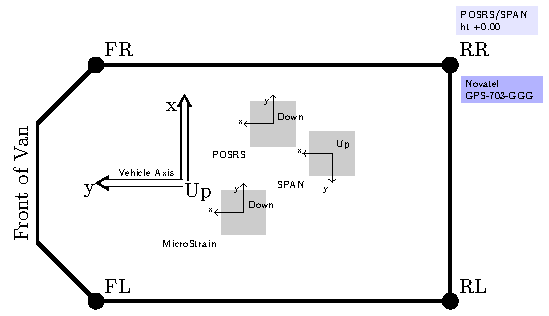
\includegraphics[clip,width=16cm]{pic/VanLayout}%%\resizebox{!}{\textheight}
\caption{Van experiment layout\label{fig:Van-experiment-layout}}
\end{figure}



\begin{table}[!htb]
\centering{}%
\begin{minipage}[t]{1\columnwidth}%
\begin{center}
\begin{tabular}{>{\centering}m{2.5cm}>{\centering}p{2cm}>{\centering}p{3cm}>{\centering}p{3cm}>{\centering}p{3cm}}
\toprule 
%\rowcolor{lightgray}
\textbf{IMU Sensor} & \multirow{2}{2cm}{\textbf{Antenna Mount}} & \multicolumn{3}{>{\centering}p{9cm}}{\textbf{Lever Arm}%
\footnote{Lever arm is estimated to the ARP. Direction IMU to antenna.}}\tabularnewline
%\rowcolor{lightgray}
 &  & X & Y & Z\tabularnewline
\midrule
\multirow{2}{2.5cm}{\textbf{POSRS}} & RR\footnote{Mount used in the trials.\label{fn:Testing-Ant}} & 0.198 & -0.830 & 0.552\tabularnewline
\cmidrule{2-5} 
 & FL & -1.134 & 2.338 & 0.557\tabularnewline
\midrule
\multirow{2}{2.5cm}{\textbf{SPAN }} & RR\textsuperscript{\ref{fn:Testing-Ant}} & 0.307 & -0.626 & 0.543\tabularnewline
\cmidrule{2-5} 
 & FL & -1.025 & 2.542 & 0.583\tabularnewline
\bottomrule
\end{tabular}\caption{Lever Arms for POSRS and SPAN\label{tab:Lever-Arm-Values}}
\par\end{center}%
\end{minipage}
\end{table}

\clearpage %to prevent jumping floats
%----------------------------------------------------------------------------------------
\section{Quality Indicators}

Inertial Explorer use colour coded Quality Indicators (IQ) to indicate quality of any positioning solution. Use it to assess the accuracy of your solution.

\begin{table}[!htb]
\centering{}%
\begin{minipage}[t]{1\columnwidth}%
\begin{center}
\begin{tabular}{>{\centering}p{2cm}>{\centering}p{3cm}>{\centering}p{6cm}>{\centering}p{3cm}}
 \rowcolor{lightgray}\textbf{QN} & \textbf{Color} & \textbf{Description} & \textbf{3D Accuracy (m) }\tabularnewline
\midrule
\textbf{1} & \textcolor{green}{Green}%
\footnote{\textbf{Recommended for LC integration}.\label{fn:Suggested-accuracy-QT}%
} & Fixed integer & $\SIrange[range-phrase=\,-\,]{0.00}{0.15}{}$\tabularnewline
\textbf{2} & \textcolor{cyan}{Cyan} \textsuperscript{\ref{fn:Suggested-accuracy-QT}} & Converged float or noisy fixed integer & $\SIrange[range-phrase=\,-\,]{0.05}{0.40}{}$\tabularnewline
\midrule
\textbf{3} & \textcolor{blue}{Blue} & Converging float & $\SIrange[range-phrase=\,-\,]{0.20}{1.00}{}$\tabularnewline
\textbf{4} & \textcolor{purple}{Purple} & Converging float & $\SIrange[range-phrase=\,-\,]{0.50}{2.00}{}$\tabularnewline
\midrule
\textbf{5} & \textcolor{magenta}{Magenta}%
\footnote{\textcolor{red}{Do not use for LC integration.}\label{fn:Not-recommended-LC}%
} & DGPS & $\SIrange[range-phrase=\,-\,]{1.00}{5.00}{}$\tabularnewline
\textbf{6} & \textcolor{red}{Red}\textsuperscript{\ref{fn:Not-recommended-LC}} & DGPS & $\SIrange[range-phrase=\,-\,]{2.00}{10.00}{}$\tabularnewline
\midrule
 & \textcolor{gray}{Grey} & Data haven't been processed & \tabularnewline
 \endrule
\end{tabular}\caption{IE Quality Number description\label{tab:Quality-Number-description}}
\par\end{center}%
\end{minipage}
\end{table}



%----------------------------------------------------------------------------------------
\section{Test route}

\begin{figure}[!htb]
\centering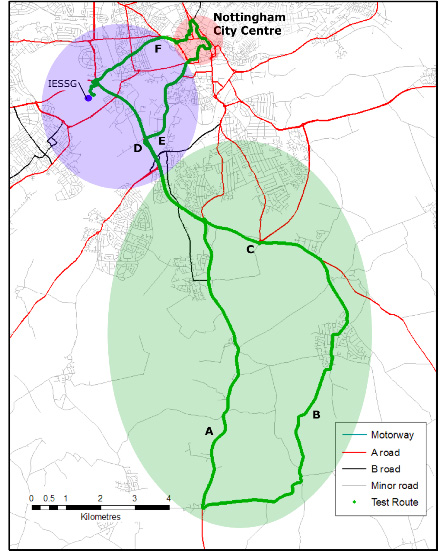
\includegraphics[clip,height=11cm]{pic/TrajectoryLayout}%%\resizebox{!}{\textheight}
\caption{Test route \label{fig:Van-trajectory}}
\end{figure}


%----------------------------------------------------------------------------------------
%HIDDEN CONTENT
%----------------------------------------------------------------------------------------
\begin{comment} 

\section{Indicative accuracy of IMUs}

Note that results below are based on small subset of data and can be treated as indicative only. Any change in movement characteristics, especially more consistent dynamics, will severely affect the outcome.


	\begin{table}[!h]
	\centering{}%
	\begin{minipage}[t]{1\columnwidth}%
	\begin{center}
	\begin{tabular}{>{\centering}p{2.5cm}c>{\centering}p{1.5cm}>{\centering}p{1cm}>{\centering}p{1cm}>{\centering}p{1cm}>{\centering}p{1cm}>{\centering}m{3cm}}
	 & \multicolumn{6}{c}{\textbf{Duration of GNSS outage {[}s{]}}%
	\footnote{Artificially generated, no valid GNSS information.%
	}} & \multirow{6}{3cm}{\begin{sideways}
	\textbf{Drift value {[}m{]}}
	\end{sideways}}\tabularnewline
	 & \multicolumn{3}{c}{\textbf{One way}} & \multicolumn{3}{c}{\textbf{Combined (Two ways)}} & \tabularnewline
	 & \textbf{56} & \textbf{92} & \textbf{401} & \textbf{56} & \textbf{92} & \textbf{401} & \tabularnewline
	\cmidrule(lr){1-1}\cmidrule(rl){2-4}\cmidrule(rl){5-7}\textbf{POSRS} & 0.30? & N/A & 6.83 & 0.30 & 1.60 & 0.91 & \tabularnewline
	\textbf{SPAN } & 0.80 & 2.90 & 127 & 0.43 & 1.50 & 6.83 & \tabularnewline
	\rowcolor{lightgray}\textbf{Microstrain} &  &  &  & 258 & 255 & 2500 & \tabularnewline
	\cmidrule{1-1} 
	\end{tabular}\caption{IMU positional drift during artificial GNSS outage, based on 2014 results}
	\par\end{center}%
	\end{minipage}
	\end{table}


\end{comment}




%----------------------------------------------------------------------------------------
%	BIBLIOGRAPHY
%----------------------------------------------------------------------------------------

% \chapter*{Bibliography}
% \addcontentsline{toc}{chapter}{\textcolor{ocre}{Bibliography}}
% \section*{Books}
% \addcontentsline{toc}{section}{Books}
% \printbibliography[heading=bibempty,type=book]
% \section*{Articles}
% \addcontentsline{toc}{section}{Articles}
% \printbibliography[heading=bibempty,type=article]

%----------------------------------------------------------------------------------------
%	INDEX
%----------------------------------------------------------------------------------------

% \cleardoublepage
% \phantomsection
% \setlength{\columnsep}{0.75cm}
% \addcontentsline{toc}{chapter}{\textcolor{ocre}{Index}}
% \printindex

%----------------------------------------------------------------------------------------

\end{document}